\documentclass[runningheads]{llncs}
\usepackage{amsmath,amssymb,booktabs,graphicx}
\usepackage{fontspec}
\usepackage{placeins}
\setmainfont{Liberation Serif}
\setlength{\tabcolsep}{3.2pt}
\renewcommand{\arraystretch}{0.9}
\setlength{\textfloatsep}{6pt plus 1pt minus 2pt}
\setlength{\intextsep}{6pt plus 1pt minus 2pt}
\setlength{\floatsep}{6pt plus 1pt minus 2pt}
\setlength{\abovecaptionskip}{4pt}
\setlength{\belowcaptionskip}{2pt}
\raggedbottom

\title{Multi-Representation Trajectory Learning for Vietnamese Air-Writing Recognition}
\author{Authors}
\institute{Institution}
\begin{document}
\maketitle

\begin{abstract}
An air-writing recognizer must learn both the geometry of a trajectory and the motion that produced it. We present a character-level Vietnamese recognizer whose learnable, time-dependent gated fusion module combines normalized spatial coordinates, dynamic kinematic descriptors, and multi-scale Fourier features. A Conformer encoder with learned clipped relative-position bias and a Connectionist Temporal Classification (CTC) objective maps the fused sequence to Vietnamese character strings. On the VNI air-writing dataset~\cite{vni} (22,754 non-duplicate trajectories, 660 labels), split source-disjointly by writer session, the validation-selected Fourier-scale $K=2$ model reaches 1.77\% character error rate (CER), 5.55\% word error rate, and 94.77\% exact sequence accuracy. Because a source-disjoint split still lets every test phrase appear verbatim in training, we additionally define a lexical-disjoint protocol with disjoint train/test phrases. There, the full architecture generalizes far worse (33.16\% CER), but dropping the spatial branch in favor of dynamics and Fourier features under stronger dropout -- with no other architectural change -- reduces this to $19.52\pm1.17\%$ CER over three seeds, evidence that the model composes characters rather than memorizing phrases. A corpus-wide analysis of the gate weights further shows genuine, curvature-dependent specialization (Spearman $\rho=0.57$ between the dynamic branch's weight and local curvature) rather than a fixed mixture.
\end{abstract}

\section{Introduction}
Air-writing recognition aims to infer characters or words directly from continuous hand or finger movements in free space~\cite{alamdepth}. This freedom of interaction also makes recognition more difficult. Without a supporting surface, small tremors readily appear in the recorded path, making preprocessing particularly important. Writing speed can also vary across instances of the same word, especially around corners and diacritics. There is no explicit pen-up signal between consecutive characters; the movement from the end of one character to the beginning of the next produces an extra stroke that the recognizer must learn to ignore.

Vietnamese adds a further source of variation. Accented vowels and tone marks may be represented by short movements that are easy to confuse with noise or with a transition stroke. A useful recognizer must therefore retain global word shape, local curvature, and the temporal behavior of the writing motion. Rendering a trajectory as one static image preserves much of its shape but can erase direction, velocity, and the ordering of overlapping strokes. We instead work directly with the coordinate sequence.

This work proposes an explicit multi-representation encoding for air-writing trajectories and evaluates it with a Conformer--CTC recognizer. Our contributions are: (i) a spatial/dynamic/Fourier trajectory representation with an adaptive, time-dependent fusion module; (ii) a lexical-disjoint evaluation protocol showing the representation choice and regularization strength -- not just architecture -- govern whether the model composes characters or memorizes phrases; and (iii) a corpus-wide, curvature-linked analysis of what the learned fusion gate actually specializes on.

\section{Related Work}
\noindent\textbf{Sensing and classical recognition.} Air-writing systems can be distinguished by how motion is acquired: wearable inertial units~\cite{airwriting}, radar range/Doppler measurements~\cite{arsalan}, or camera-based fingertip/hand-landmark tracking~\cite{alamdepth,watanabe}. The VNI collection belongs to the last category, providing 2D coordinate sequences rather than raw video. Early pipelines used handcrafted descriptors (angles, velocity, curvature, turning points) with dynamic time warping, hidden Markov models, or shallow classifiers~\cite{rumelhart} on fixed-length feature vectors -- inexpensive but sensitive to scale, orientation, and style variation.

\noindent\textbf{Image-based and spatio-temporal convolution.} Rasterizing a trajectory and recognizing it with a CNN~\cite{alamcnn,lamaakal,roy} learns spatial shape well but a static rendering loses stroke direction, velocity, and overlap ordering; coloring strokes by time or stacking a temporal tensor dimension~\cite{chang,kimst} preserves more timing at the cost of sparse, higher-dimensional inputs. We avoid rasterization and operate directly on the ordered coordinate sequence.

\noindent\textbf{Sequence models: RNN, Transformer, Conformer.} RNN/LSTM encoders~\cite{rumelhart,hochreiter,ott} model handwriting dynamics but limit parallelism and long-range interaction; Transformer time-series models replace recurrence with self-attention~\cite{zerveas,zheng} but do not explicitly emphasize the short local motion patterns around corners and epenthetic strokes. The Conformer combines multi-head self-attention with depthwise convolution in a Macaron layout~\cite{conformer}, matching air-writing's mix of global phrase structure and local direction/curvature change. We evaluate recurrent, temporal-convolutional, Transformer, and Conformer backbones under an identical protocol, and add learned relative-position bias so attention depends on temporal distance rather than a fixed absolute index.

\noindent\textbf{CTC and Fourier features.} Connectionist Temporal Classification~\cite{ctc} sums over frame-level paths that collapse to a target string, avoiding manual character segmentation -- appropriate here since a trajectory and its text label carry no explicit alignment. Random Fourier Features~\cite{fourier} project coordinates into $[\sin(2\pi Bp),\cos(2\pi Bp)]$ to counter the spectral bias of MLPs toward low frequencies, exposing small curves, direction changes, and diacritic strokes that raw coordinates represent poorly. We use a deterministic dyadic frequency bank $2^k\pi$ instead of a sampled Gaussian matrix, keeping the mapping reproducible and enabling a controlled ablation over the scale count $K$.

\section{Methodology}
\subsection{Dataset and Evaluation Protocol}
\label{sec:protocol}
We use the VNI air-writing collection~\cite{vni}, one of the few public trajectory datasets designed for Vietnamese. Each sample is a CSV of ordered fingertip coordinates $(x,y)$, preserving stroke order, speed, hesitation, and transition movements that a static image would lose. The 22,760 trajectories span four groups: 15,500 samples over 310 one-word labels, 5,760 over 200 two-word labels, 500 over 50 three-word labels, and 1,000 over 100 longer phrases.

Recognition operates at the character level even though directory labels are words or phrases: the alphabet has 86 non-space characters plus one explicit space, and the CTC blank gives 88 output classes in total. This lets one model transcribe both isolated words and multi-word phrases without treating every phrase as its own class.

Our primary protocol is \emph{source-disjoint}: numeric source IDs are shuffled and partitioned globally into 40 training, 5 validation, and 5 test IDs, so every one of the 660 labels appears in every split, but with disjoint recording sessions. This protocol does not, however, rule out phrase-level memorization, since every test phrase was still seen verbatim during training. We therefore also define a \emph{lexical-disjoint} protocol (Section~\ref{sec:lexical}): complete labels are stratified by phrase-length group and split 80/10/10 so that none of the 66 test phrases occur among the 528 training phrases, while every evaluation character still occurs in at least one training label.

\subsection{Trajectory Preprocessing and Multi-Representation Features}
Given $P=\{p_t=(x_t,y_t)\}_{t=1}^{T}$, we remove consecutive near-duplicate points, apply a Savitzky--Golay filter (odd window $\le7$, third-order) to each coordinate, and interpolate both with cubic splines on a denser grid. Position and scale are then normalized by centroid and maximum radial distance,
\begin{equation}
\bar p=\frac{1}{T}\sum_{t=1}^{T}p_t,\qquad
\hat p_t=\frac{p_t-\bar p}{\max_j\lVert p_j-\bar p\rVert_2},
\end{equation}
preserving aspect ratio while removing translation and global scale. We compute cumulative arc length $s_1=0,\ s_t=\sum_{j=2}^{t}\lVert \hat p_j-\hat p_{j-1}\rVert_2$ and resample the curve at $L$ equally spaced arc-length positions ($L=128$ by default; $L\in\{64,96,128,192,256\}$ ablated). The same function is used for training, evaluation, robustness testing, and inference.

The spatial branch is $S_t=[x_t,y_t]$. The dynamic branch $D_t=[\Delta x_t,\Delta y_t,v_t,d^x_t,d^y_t,a_t,\kappa_t]$ collects first differences, arc-length speed $v_t$, unit tangent direction $d_t$, speed difference $a_t$, and clipped signed curvature $\kappa_t$ -- local geometric-motion descriptors rather than raw temporal speed, since arc-length resampling equalizes spacing along the curve. The Fourier branch $F_t=[\sin(2^k\pi p_t),\cos(2^k\pi p_t)]_{p\in\{x,y\},\,k=0}^{K-1}$ has $4K$ dimensions per step; we evaluate $K\in\{2,4,6,8\}$.

\subsection{Training-Only Data Augmentation}
Training trajectories (only) are augmented once, after preprocessing, with four transformations: rotation $p'_t=R(\theta)p_t,\ \theta\sim\mathcal U(-15^\circ,15^\circ)$, modeling wrist/camera orientation change; independent axis stretching $x'_t=s_xx_t,\ y'_t=s_yy_t,\ s_x,s_y\sim\mathcal U(0.85,1.15)$, modeling aspect-ratio variation; additive noise $p'_t=p_t+\epsilon_t,\ \epsilon_t\sim\mathcal N(0,0.008^2I)$, modeling tremor and tracking error; and temporal warping, where positive increments $q_t=\exp(z_t),\ z_t\sim\mathcal N(0,0.2^2)$ are accumulated into a monotone time axis and interpolated, stretching some intervals and compressing others without reordering points. Validation and test trajectories are left untouched, since augmenting them would duplicate evaluation examples and bias reported metrics.

\begin{figure}[htbp]
\centering
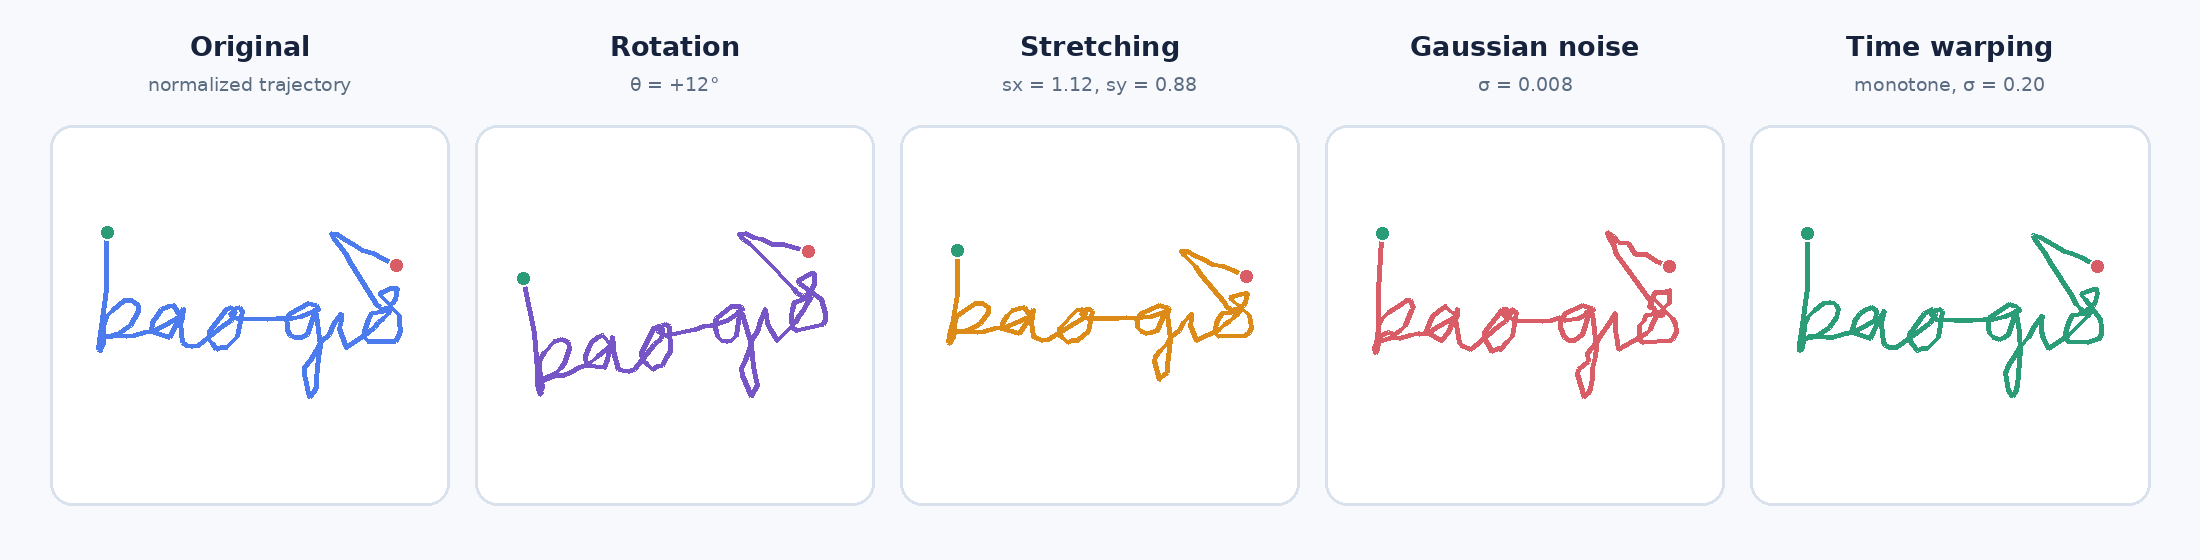
\includegraphics[width=0.7\linewidth]{figures/training_augmentation.png}
\caption{Augmentation applied to a normalized trajectory. Green/red markers denote the first/last points.}
\label{fig:augmentation}
\end{figure}

\subsection{Proposed Model Architecture}
Each available branch is independently embedded by $\mathrm{Linear}\rightarrow\mathrm{LayerNorm}\rightarrow\mathrm{SiLU}$ into $d=128$ dimensions (Figure~\ref{fig:architecture}). For gated fusion, branch weights are predicted at every time step,
\begin{equation}
\alpha_t=\operatorname{softmax}(W[h_t^S;h_t^D;h_t^F]),\qquad
h_t=\sum_{b\in\{S,D,F\}}\alpha_t^b h_t^b,
\end{equation}
letting the model select the most informative representation locally instead of always concatenating all branches.

The fused sequence passes through four Conformer blocks (four heads, $d_{\mathrm{model}}=128$, feed-forward width 512, dropout 0.1, depthwise convolution kernel 15) in the Macaron layout: half-step feed-forward, self-attention, convolution, half-step feed-forward, with residuals and layer norm. Relative self-attention adds a learned head-specific bias indexed by clipped distance $j-i\in[-64,64]$: $A_{ij}=Q_iK_j^T/\sqrt{d_h}+b_{\mathrm{clip}(j-i)}$. The encoder output projects to 88 classes with log-softmax, trained with
\begin{equation}
\mathcal L_{\mathrm{CTC}}=-\log\sum_{\pi\in\mathcal B^{-1}(y)}\prod_{t=1}^{L}P(\pi_t\mid h_t),
\end{equation}
where $\mathcal B^{-1}(y)$ is the set of frame-level paths collapsing to target string $y$ (removing blanks, merging repeats), so explicit character boundaries are unnecessary while the space token stays available for multi-word labels. The selected configuration is the gated relative-position Conformer with all three branches and Fourier scale $K=2$.

\begin{figure}[htbp]
\centering
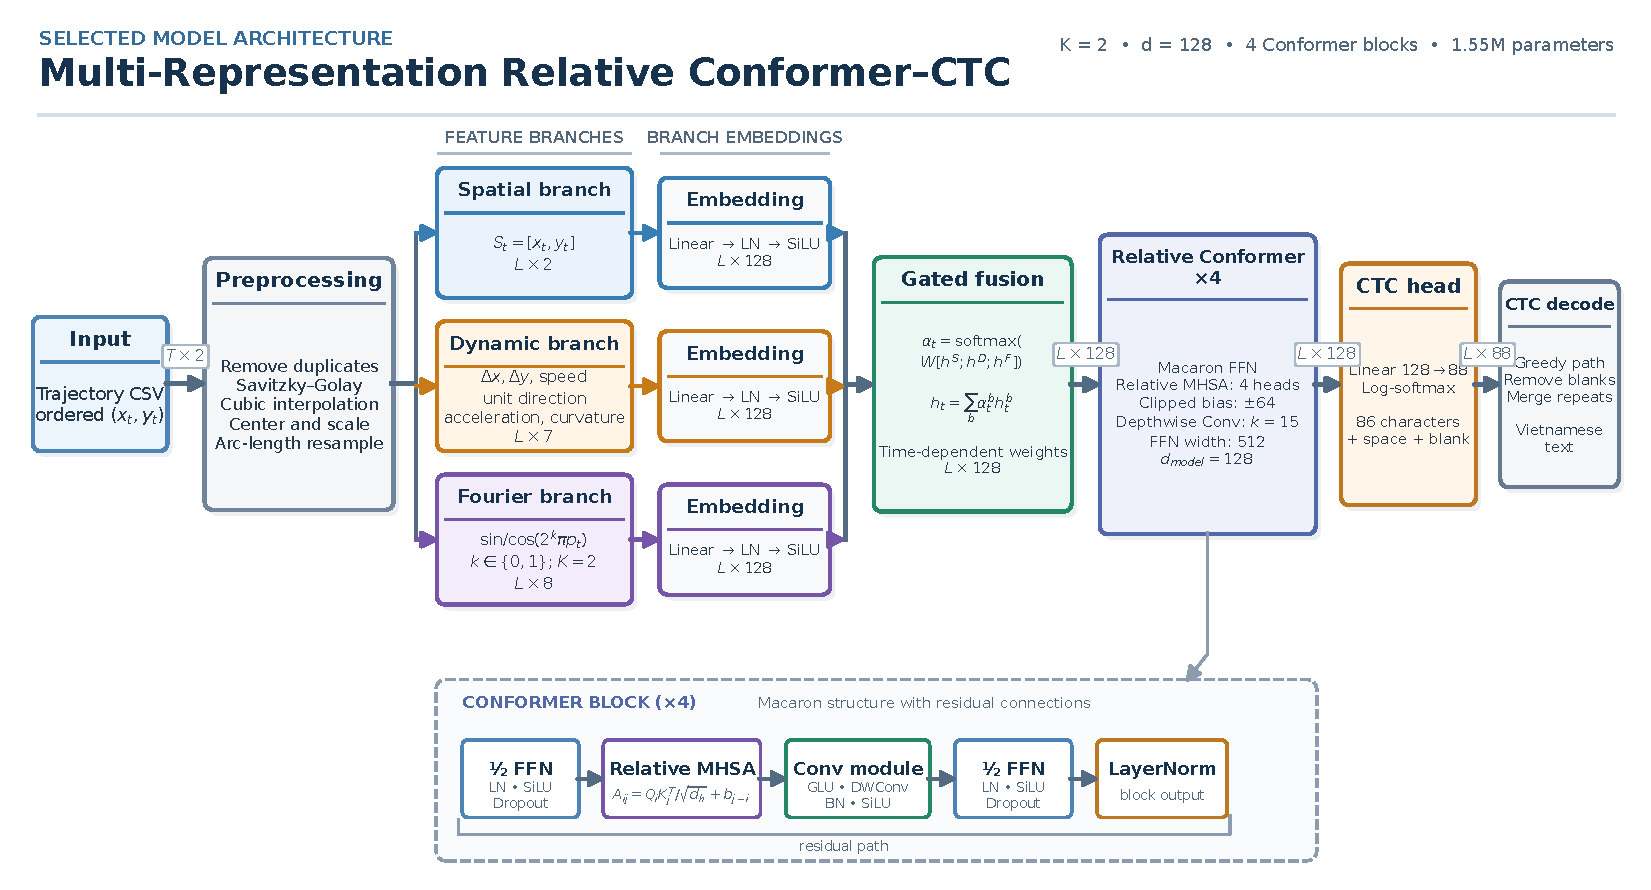
\includegraphics[width=0.75\linewidth]{figures/best_model_architecture.pdf}
\caption{Architecture used in the reproducible experiments.}
\label{fig:architecture}
\end{figure}

\section{Experimental Setup}
We train with AdamW, initial learning rate $10^{-3}$, four-epoch linear warm-up then cosine decay, weight decay $10^{-2}$, batch size 512, gradient-norm clipping at 5, at most 40 epochs, and early stopping after 20 epochs without validation-CER improvement; the lowest-validation-CER checkpoint is evaluated on the test set. The core suite compares BiLSTM, GRU, TCN, Transformer, and Conformer backbones; spatial/dynamic/Fourier representations; concatenation/sum/static/gated fusion; none/absolute/relative positional encoding; and augmentation on/off. The extended suite varies Fourier scale, preprocessing, and resampling length. Robustness evaluation applies rotation, additive noise, scale, and temporal-warp perturbations to the selected checkpoint. All experiments use the frozen source-disjoint manifest and seed 42 unless a multi-seed confirmation is explicitly reported. We report CER $=(S+D+I)/N$, WER, exact sequence accuracy, and insertion/deletion/substitution counts, computed on Unicode NFC-normalized strings with spaces preserved.

A separate lexical-disjoint experiment (Section~\ref{sec:lexical}) uses the frozen lexical-disjoint manifest of Section~\ref{sec:protocol} instead, with augmentation disabled throughout. It first trains the default full architecture (S+D+F, gated fusion, dropout 0.1) with and without augmentation, then a leaner D+F, concatenation-fusion model at dropout $\in\{0.1,0.2,0.3,0.4\}$, then two controls that isolate branch dropout and full-architecture dropout as alternative explanations. The best configuration by validation CER (D+F, dropout 0.2) is retrained at three seeds (42, 3407, 2026) with the manifest held fixed, so seed variation is not conflated with split variation.

\section{Results}
Tables~\ref{tab:backbone}--\ref{tab:robustness} report source-disjoint results; S, D, F denote the spatial, dynamic, and Fourier branches. Validation CER is the checkpoint-selection criterion; test CER/WER/exact accuracy are reported only after selection. The nominal $K=4$ configuration was run independently in the core and extended suites (2.40\% vs.\ 2.36\% test CER); we retain both as a rerun sanity check.

\subsection{Backbone Comparison}
\begin{table}[htbp]
\centering
\caption{Backbone comparison at seed 42. All rows use S+D features, concatenation, augmentation, $L=128$. TCN is a reduced diagnostic (Section~\ref{sec:protocol} setup), not a fair-capacity comparison.}
\label{tab:backbone}
\begin{tabular}{llrrrr}
\toprule
Backbone & PE & Params (M) & CER (\%) & WER (\%) & Exact (\%)\\
\midrule
BiLSTM & None & 0.443 & 73.58 & 97.55 & 3.51\\
GRU & None & 0.344 & 58.58 & 92.55 & 10.63\\
TCN (reduced) & None & 0.098 & 91.02 & 100.00 & 0.00\\
Transformer & Absolute & 0.839 & 11.79 & 22.51 & 85.85\\
Conformer & Relative & 1.579 & \textbf{1.85} & \textbf{5.46} & \textbf{94.90}\\
\bottomrule
\end{tabular}
\end{table}

A three-seed confirmation (42, 43, 44) on the source-disjoint split shows this ranking is stable: BiLSTM $74.30\pm0.85\%$, Transformer + absolute PE $14.76\pm2.77\%$, Conformer + relative PE $1.94\pm0.11\%$, and the gated S+D+F, $K=4$ configuration $2.48\pm0.18\%$ CER (mean $\pm$ sample standard deviation).

\subsection{Representation and Fusion Ablations}
\begin{table}[htbp]
\centering
\caption{Representation ablation at seed 42. Relative-position Conformer, concatenation fusion; Fourier rows use $K=4$. $\Delta$ is $(\Delta x,\Delta y)$ only; D is all seven dynamic descriptors.}
\label{tab:representation}
\resizebox{\linewidth}{!}{%
\begin{tabular}{llrrrrrr}
\toprule
Representation & Features & Params (M) & Epoch & Val. CER (\%) & CER (\%) & WER (\%) & Exact (\%)\\
\midrule
Coordinates & S & 1.544 & 40 & 3.13 & 3.22 & 8.77 & 92.62\\
Coordinates + displacement & S+$\Delta$ & 1.578 & 37 & 3.05 & 3.03 & 8.49 & 93.37\\
Dynamics only & D & 1.546 & 38 & 3.19 & 3.20 & 8.61 & 92.75\\
Fourier only & F & 1.546 & 38 & 5.72 & 5.67 & 13.52 & 89.67\\
Coordinates + Fourier & S+F & 1.580 & 38 & 4.84 & 4.13 & 11.59 & 91.34\\
Dynamics + Fourier & D+F & 1.580 & 37 & \textbf{1.68} & \textbf{1.77} & \textbf{5.37} & 94.33\\
Coordinates + dynamics & S+D & 1.579 & 39 & 2.05 & 1.85 & 5.46 & \textbf{94.90}\\
All (S+D+F), concat. & S+D+F & 1.597 & 38 & 2.12 & 2.23 & 6.41 & 94.42\\
\bottomrule
\end{tabular}}
\end{table}

\begin{table}[htbp]
\centering
\caption{Fusion ablation at seed 42, S+D+F, relative-position Conformer, $K=4$. Static fusion learns one global branch-weight vector; gated fusion predicts branch weights per time step.}
\label{tab:fusion}
\resizebox{\linewidth}{!}{%
\begin{tabular}{lrrrrrr}
\toprule
Fusion & Params (M) & Epoch & Val. CER (\%) & CER (\%) & WER (\%) & Exact (\%)\\
\midrule
Concatenation & 1.597 & 38 & \textbf{2.12} & 2.23 & \textbf{6.41} & \textbf{94.42}\\
Sum & 1.548 & 40 & 2.24 & \textbf{2.22} & 6.99 & 93.50\\
Static weights & 1.548 & 40 & 2.22 & 2.36 & 7.21 & 93.59\\
Time-dependent gate & 1.549 & 40 & 2.18 & 2.40 & 6.93 & 93.94\\
\bottomrule
\end{tabular}}
\end{table}

Under simple concatenation, adding the third branch does not help monotonically (D+F: 1.77\%; S+D+F: 2.23\%), which motivates a fusion mechanism able to down-weight a less useful branch rather than always concatenating all three; Section~\ref{sec:lexical} and the gate analysis below return to this point under the harder lexical-disjoint protocol, where the choice between these representations changes the outcome by more than a factor of 1.5.

\subsection{Positional Encoding, Augmentation, and Secondary Ablations}
Table~\ref{tab:secondary} isolates positional encoding and augmentation, then extends to Fourier scale, preprocessing, and resampling length, all at the shared $K=4$, S+D+F, gated-fusion default unless the block itself varies that factor.

\begin{table}[htbp]
\centering
\caption{Positional-encoding, augmentation, Fourier-scale, preprocessing, and resampling-length ablations at seed 42. Unless the block itself varies the factor, all rows use S+D+F, gated fusion, $K=4$, relative PE, and default preprocessing/length. ``Raw'' disables smoothing, spline interpolation, and normalization.}
\label{tab:components}
\label{tab:secondary}
\resizebox{\linewidth}{!}{%
\begin{tabular}{llrrrrr}
\toprule
Study & Setting & Epoch & Val. CER (\%) & CER (\%) & WER (\%) & Exact (\%)\\
\midrule
PE & None & 40 & \textbf{2.16} & \textbf{1.74} & \textbf{5.52} & \textbf{94.82}\\
PE & Absolute & 38 & 4.74 & 4.12 & 10.30 & 91.83\\
PE & Relative & 40 & 2.18 & 2.40 & 6.93 & 93.94\\
\midrule
Augmentation & Disabled & 39 & \textbf{1.51} & \textbf{1.57} & \textbf{4.97} & \textbf{94.64}\\
Augmentation & Enabled & 40 & 2.18 & 2.40 & 6.93 & 93.94\\
\midrule
Fourier scale & $K=2$ & 38 & \textbf{1.85} & \textbf{1.77} & \textbf{5.55} & \textbf{94.77}\\
Fourier scale & $K=4$ & 40 & 2.24 & 2.36 & 7.11 & 93.28\\
Fourier scale & $K=6$ & 40 & 2.17 & 2.13 & 6.69 & 93.67\\
Fourier scale & $K=8$ & 36 & 2.31 & 2.14 & 6.53 & 93.85\\
\midrule
Preprocessing & Raw & 39 & 2.16 & 2.33 & 6.93 & 94.11\\
Preprocessing & Savitzky--Golay & 40 & 2.16 & 2.01 & 6.32 & 94.11\\
Preprocessing & Spline & 38 & \textbf{1.92} & \textbf{1.72} & \textbf{5.61} & \textbf{94.86}\\
Preprocessing & Full (SG + spline) & 40 & 2.24 & 2.36 & 7.11 & 93.28\\
\midrule
Length & $L=64$ & 39 & 2.81 & 2.82 & 7.33 & \textbf{94.07}\\
Length & $L=96$ & 35 & 2.49 & 2.34 & 6.87 & 94.02\\
Length & $L=128$ & 40 & 2.24 & 2.36 & 7.11 & 93.28\\
Length & $L=192$ & 36 & \textbf{2.12} & \textbf{1.94} & \textbf{6.35} & 93.72\\
\bottomrule
\end{tabular}}
\end{table}

\FloatBarrier
\subsection{Robustness}
\begin{table}[htbp]
\centering
\caption{Robustness of the selected $K=2$ checkpoint. Rotation (signed, degrees) is applied symmetrically about $0^\circ$ since a camera/wrist offset has no preferred direction; noise is normalized coordinate standard deviation; scale is multiplicative; time warp is the log-increment standard deviation.}
\label{tab:robustness}
\resizebox{\linewidth}{!}{%
\begin{tabular}{lrrrr}
\toprule
Perturbation & Strength & CER (\%) & WER (\%) & Exact (\%)\\
\midrule
Rotation & $-20$ & 3.67 & 10.92 & 89.54\\
Rotation & $-10$ & 2.03 & 6.59 & 93.80\\
Rotation & $0$ & 1.77 & 5.55 & 94.77\\
Rotation & $10$ & 2.23 & 6.96 & 93.76\\
Rotation & $20$ & 3.50 & 10.40 & 89.98\\
\midrule
Noise & 0 & 1.77 & 5.55 & 94.77\\
Noise & 0.005 & 1.80 & 5.49 & 94.86\\
Noise & 0.010 & 2.50 & 7.61 & 92.88\\
Noise & 0.020 & 8.74 & 22.82 & 79.04\\
Noise & 0.050 & 50.73 & 90.40 & 20.12\\
\midrule
Scale & 0.8 & 2.38 & 7.48 & 93.01\\
Scale & 1.0 & 1.77 & 5.55 & 94.77\\
Scale & 1.2 & 2.27 & 6.99 & 93.85\\
\midrule
Time warp & 0 & 1.77 & 5.55 & 94.77\\
Time warp & 0.20 & 2.06 & 6.13 & 94.11\\
Time warp & 0.35 & 2.87 & 8.34 & 92.49\\
\bottomrule
\end{tabular}}
\end{table}
Degradation is close to symmetric under rotation (3.67\% CER at $-20^\circ$ vs.\ 3.50\% at $+20^\circ$), indicating no directional bias in what the model has learned. CER stays below 3\% within $\pm15^\circ$ rotation, over scales 0.8--1.2, and at time-warp strength 0.35. Coordinate noise is far more damaging, rising from 2.50\% CER at $\sigma=0.01$ to 50.73\% at $\sigma=0.05$: the system tolerates geometric and timing variation better than severe fingertip-localization noise.

\subsection{Lexical-Disjoint Generalization}
\label{sec:lexical}
The source-disjoint protocol still allows every test label to have been seen, worded identically, during training. Table~\ref{tab:lexical} instead uses the lexical-disjoint protocol of Section~\ref{sec:protocol}, where none of the 66 test phrases occur in the 528 training phrases. All rows use the same Conformer backbone, relative-position bias, and CTC objective as the main experiments, with augmentation disabled throughout (Table~\ref{tab:components} already shows augmentation is not beneficial even in the easier source-disjoint setting).

\begin{table}[htbp]
\centering
\caption{Lexical-disjoint open-phrase recognition (66 unseen test phrases). All rows disable augmentation, relative-position Conformer; D+F rows use dynamics+Fourier concatenation, batch size 256. ``Full model, control'' applies the same dropout to the default S+D+F gated architecture instead of removing the spatial branch.}
\label{tab:lexical}
\resizebox{\linewidth}{!}{%
\begin{tabular}{llrrrr}
\toprule
Configuration & Dropout & Params (M) & Epoch & Val. CER (\%) & CER (\%)\\
\midrule
Full model (S+D+F, gated) & 0.1 & 1.548 & 38 & 34.06 & 33.16\\
\quad -- augmentation disabled & 0.1 & 1.549 & 32 & 28.48 & 31.99\\
D+F, concatenation & 0.1 & 1.580 & 30 & 31.18 & 31.82\\
\midrule
D+F, concatenation & 0.2 & 1.580 & 65 & \textbf{18.39} & \textbf{20.86}\\
D+F, concatenation & 0.3 & 1.580 & 29 & 19.38 & 24.22\\
D+F, concatenation & 0.4 & 1.580 & 63 & 18.66 & 23.04\\
D+F, concat.\ + branch dropout 0.2 & 0.3 & 1.580 & 49 & 22.28 & 25.78\\
Full model (S+D+F, gated), control & 0.3 & 1.549 & 64 & 25.37 & 26.05\\
\bottomrule
\end{tabular}}
\end{table}

Two effects are visible and separable. First, representation choice matters on its own: at the default dropout of 0.1, dropping the spatial branch (D+F, 31.82\% CER) is roughly as good as keeping it (31.99\% CER), so the spatial branch contributes little to lexical generalization even before extra regularization -- consistent with it mainly encoding absolute phrase shape, which does not transfer to an unseen phrase. Second, regularization strength matters a great deal for D+F specifically: raising dropout from 0.1 to 0.2 nearly halves CER (31.82\%$\to$20.86\%). Applying the same dropout of 0.3 to the full gated S+D+F architecture instead (``control'') only reaches 26.05\% CER, worse than D+F at any tested dropout -- so the gain is not simply ``more dropout helps,'' but specifically favors the leaner representation once regularized. Stacking branch dropout on top of dropout 0.3 (25.78\%) does not improve on plain dropout at 0.2--0.3, so we do not pursue further regularization axes. We confirm the winning configuration (D+F, dropout 0.2) across three seeds (42, 3407, 2026): CER $19.52\pm1.17\%$, WER $52.39\pm2.02\%$, exact accuracy $37.16\pm3.05\%$. The overall result is a reduction from 33.16\% to $19.52\pm1.17\%$ CER (13.6 points absolute, 41\% relative) on completely unseen phrases, using the same Conformer-CTC architecture and only a representation and dropout change.

To test whether the gated fusion module genuinely specializes rather than converging to a fixed mixture, we extract per-time-step gate weights $\alpha_t=(\alpha_t^S,\alpha_t^D,\alpha_t^F)$ for every valid point of every source-disjoint test trajectory using the selected $K=2$ checkpoint (291{,}328 points, 2{,}276 trajectories), and compute the corpus-wide mean weight per branch, the normalized entropy $H_t=-\sum_b\alpha_t^b\log\alpha_t^b/\log 3\in[0,1]$ (0: one-hot, 1: uniform), the fraction of points at which each branch ``wins,'' and the Spearman correlation between $|\kappa_t|$ and each branch's weight.

\begin{table}[htbp]
\centering
\caption{Gate specialization for the selected $K=2$ checkpoint, over every point of every test trajectory. ``Wins'' is the fraction of points where a branch gets the largest weight. All three $\rho$ have $p<10^{-6}$.}
\label{tab:gate}
\begin{tabular}{lrrr}
\toprule
Branch & Mean weight & Wins (\%) & $\rho(|\kappa|,\alpha)$\\
\midrule
Spatial (S) & 0.196 & 5.80 & $-0.311$\\
Dynamic (D) & 0.360 & 42.08 & $\mathbf{0.571}$\\
Fourier (F) & 0.444 & 52.11 & $-0.242$\\
\bottomrule
\end{tabular}
\end{table}

All three branches win a non-trivial share of points (spatial: 5.80\%), so the gate does not collapse onto one representation, and mean normalized entropy is $0.890\pm0.118$, below the uniform value of 1. Most informative is the curvature correlation: the dynamic branch's weight rises with $|\kappa_t|$ ($\rho=0.571$) while spatial and Fourier weights fall ($\rho=-0.311,-0.242$) -- at geometrically complex points (corners, diacritic strokes, direction reversals) the model shifts weight toward the branch that most directly encodes instantaneous motion, relying more on global shape and periodic detail along straighter segments. This gives a quantitative, corpus-wide counterpart to the single-example gate curves in Figure~\ref{fig:qualitative-long}.

\subsection{Quantitative and Qualitative Analysis}
The selected $K=2$ model produces 207 character-level edit operations over 11,721 reference characters (101 substitutions, 81 deletions, 25 insertions; CER 1.77\%) and 181 word-level errors over 3,261 reference words (WER 5.55\%); 2,157 of 2,276 test trajectories are transcribed exactly (94.77\%). The relative-position Conformer reduces CER from 11.79\% (Transformer) to 1.85\%, confirmed over three seeds ($1.94\pm0.11\%$ vs.\ $14.76\pm2.77\%$); recurrent baselines remain far weaker. The component ablations (Table~\ref{tab:secondary}) show no single factor dominates in isolation -- no positional encoding and disabled augmentation both beat the default configuration alone -- so the $K=2$ checkpoint's accuracy should be attributed to the joint configuration rather than any one component; length $L=192$ and spline-only preprocessing each individually improve on the $K=4$ default, suggesting headroom the selected checkpoint does not yet capture.

Figure~\ref{fig:qualitative-bao-gio} plots each example's preprocessed trajectory (colored by time, green/red markers denoting the first/last point) above its three per-time-step gate curves $\alpha_t^S,\alpha_t^D,\alpha_t^F$. \emph{Bao giờ} (left, 156 raw points) and the harder 415-point phrase \emph{ngọn núi cao vời vợi} (center) are both decoded exactly, with mean spatial/dynamic/Fourier gate weights $0.181/0.409/0.411$ and $0.162/0.454/0.384$ respectively -- no single branch dominates throughout, consistent with the corpus-wide gate analysis above. The right panel shows a failure case: \emph{bí} decoded as \emph{bú}, a base-vowel substitution rather than a segmentation error (length and tone mark are retained). Its gate curve makes the failure mechanistically visible: the Fourier weight spikes sharply (to ${\approx}0.8$) exactly over the short vowel-defining stroke around the trajectory's midpoint, the same brief movement whose weakening under smoothing and resampling plausibly causes the \emph{i}/\emph{u} confusion. Samples with two to seven non-space characters have CER 0.31--0.48\%, but samples with eight or more rise to 4.59\% and contribute 178 of the 207 character errors -- long trajectories remain the principal failure mode even though all inputs are compressed to the same 128-point representation.

\begin{figure}[htbp]
\centering
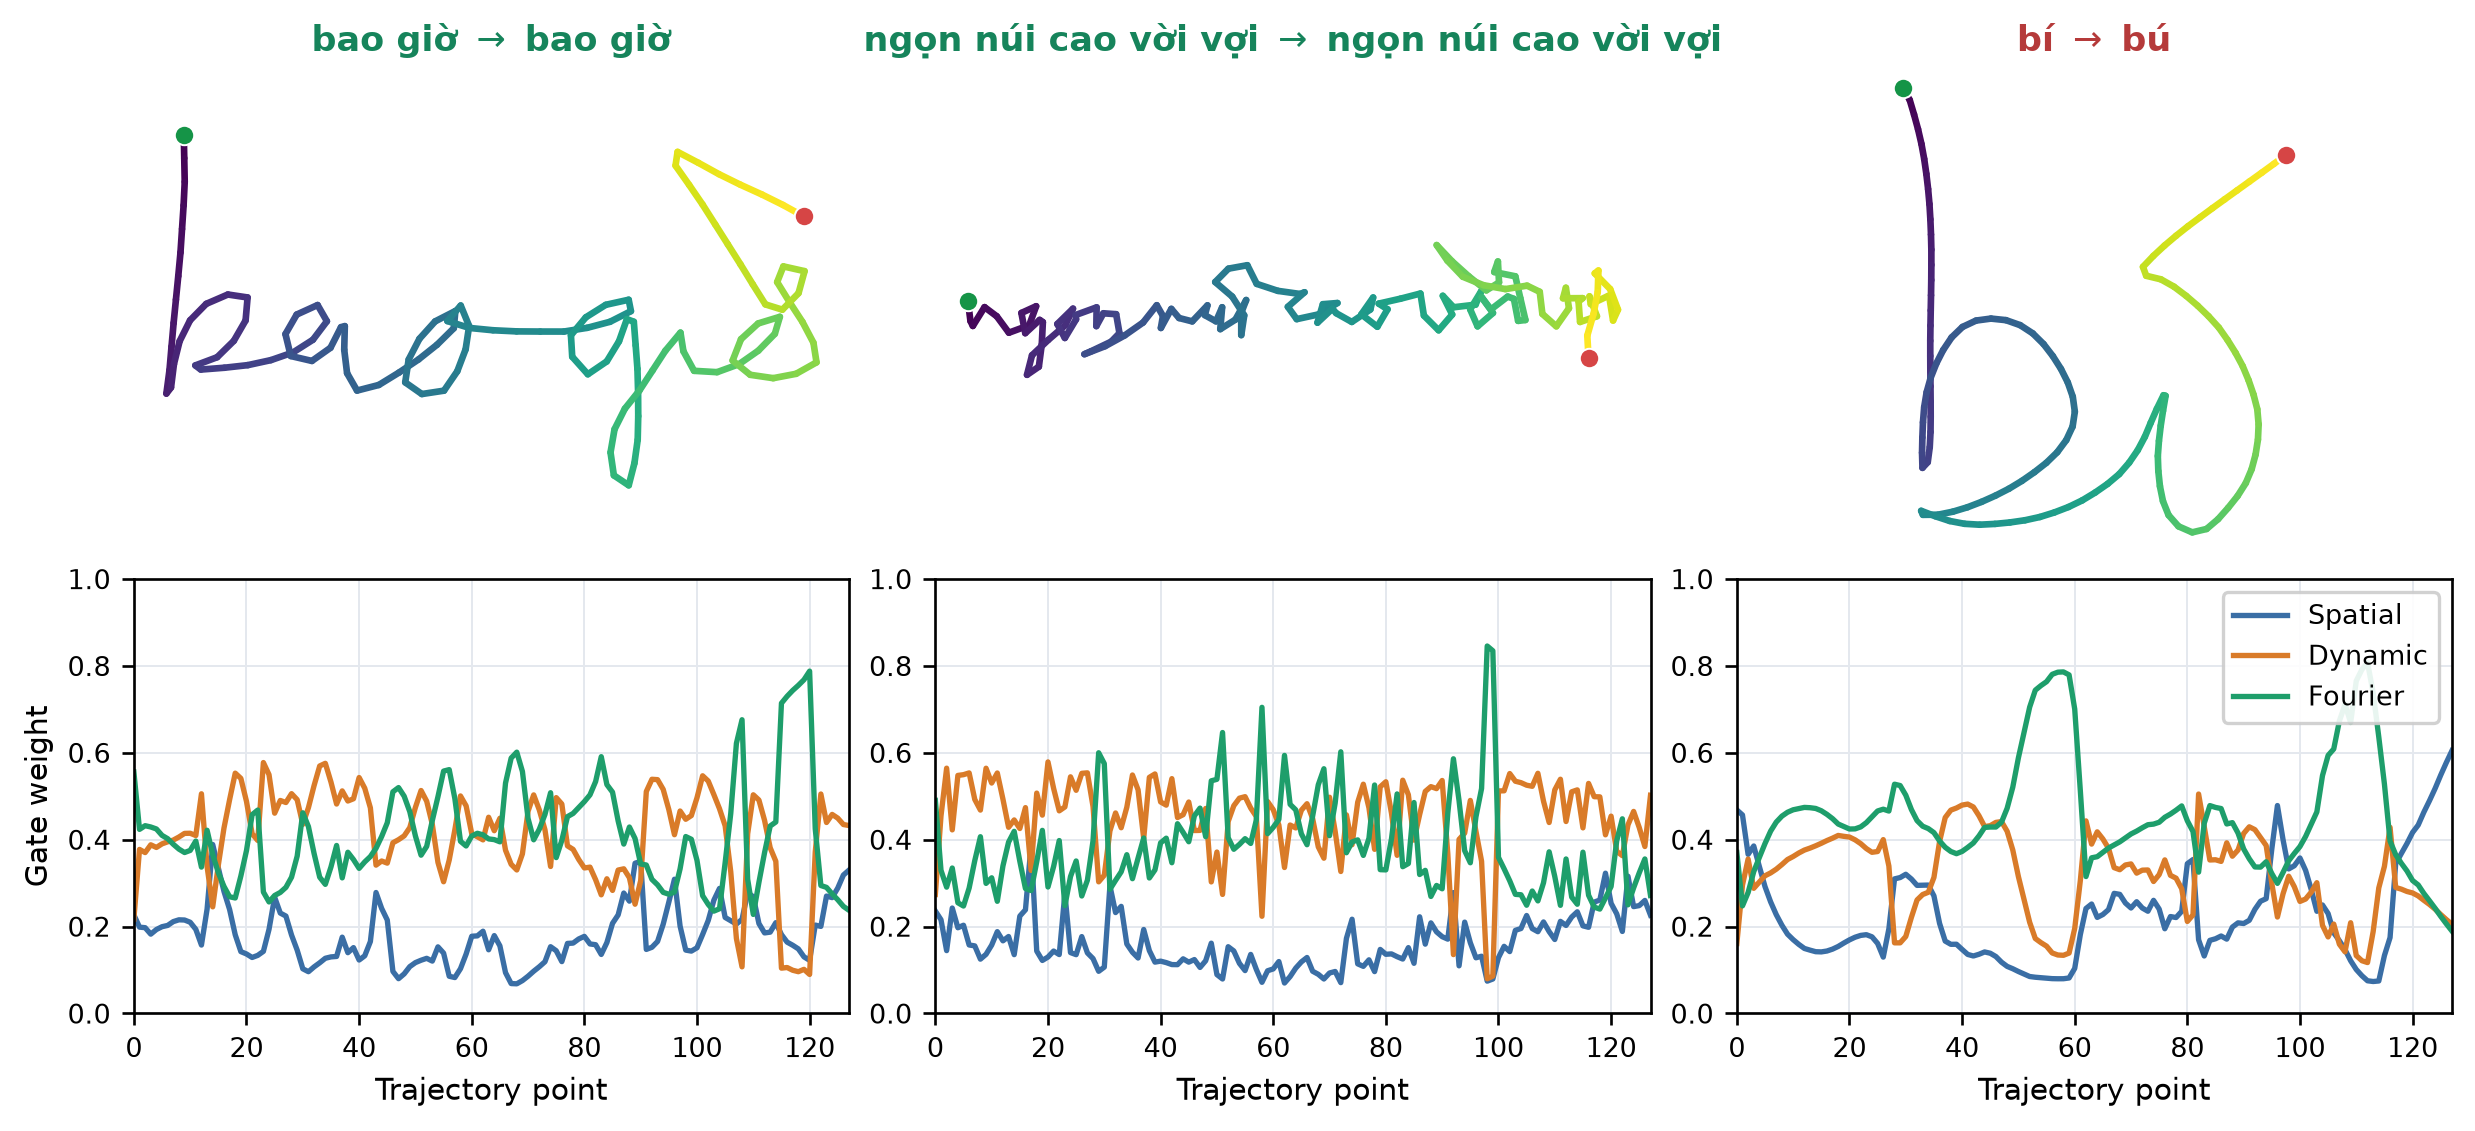
\includegraphics[width=\linewidth]{figures/gate_curves.png}
\caption{Top: preprocessed trajectory (color = time; green/red = first/last point) for \emph{bao giờ} (left, correct), \emph{ngọn núi cao vời vợi} (center, correct), and \emph{bí}$\to$\emph{bú} (right, failure). Bottom: the corresponding per-time-step gate weights $\alpha_t^S,\alpha_t^D,\alpha_t^F$ predicted by the fusion module.}
\label{fig:qualitative-bao-gio}
\label{fig:qualitative-long}
\label{fig:qualitative-bi}
\end{figure}

\subsection{Vietnamese Orthographic Error Analysis}
The \emph{bí}$\to$\emph{bú} example suggests some errors change the base vowel while leaving the tone mark intact. To quantify this across the full test set, we decompose every reference and hypothesis character via Unicode NFD normalization into a base letter and combining marks (e.g.\ \emph{\'i} $\to$ base \emph{i} + acute mark), and classify each non-correct edit from the $K=2$ checkpoint's alignments into base-character, diacritic/tone, space, deletion, or insertion.

\begin{table}[htbp]
\centering
\caption{Vietnamese orthographic error taxonomy, $K=2$ checkpoint, all 207 test-set character errors (11{,}721 reference characters).}
\label{tab:taxonomy}
\begin{tabular}{lrr}
\toprule
Error type & Count & \% of errors\\
\midrule
Base-character substitution & 84 & 40.58\\
Deletion & 81 & 39.13\\
Insertion & 25 & 12.08\\
Diacritic/tone substitution & 15 & 7.25\\
Space & 2 & 0.97\\
\bottomrule
\end{tabular}
\end{table}
Base-character confusions (40.58\%) outnumber diacritic/tone confusions (7.25\%) by more than five to one. Residual errors concentrate in distinguishing base-letter shapes -- such as the short, low-amplitude strokes separating \emph{i} and \emph{u} -- rather than in placing Vietnamese tone marks, which correspond to more distinctive secondary strokes. Combined with the length analysis above, future improvements should target short discriminative sub-strokes generally, not diacritic placement specifically.

\FloatBarrier
\section{Limitation}
The model recognizes tracked 2D trajectories; it does not detect fingertips from images or video, so reported metrics exclude errors from lighting, viewpoint, occlusion, or upstream hand tracking. Long trajectories and short discriminative vowel/diacritic movements remain the main failure modes, and the lexical-disjoint protocol still draws its 66 test phrases from the same 86-character alphabet seen in training.

\section{Future Work}
Extending the vocabulary and balancing rare Vietnamese characters would make the diacritic analysis more reliable. An end-to-end model operating on video could jointly learn fingertip tracking and transcription, requiring substantially more annotated data. Language-model rescoring could help recover missing spaces and implausible character sequences, and the length- and preprocessing-ablation results (Table~\ref{tab:secondary}) suggest $L=192$ and spline-only smoothing are worth combining with the gated architecture in future work.

\section{Conclusion}
We converted Vietnamese air-writing recognition into a reproducible source-disjoint sequence experiment and then stress-tested its central claim with a lexical-disjoint protocol. The final model combines spatial, dynamic, and Fourier trajectory representations through adaptive gated fusion with a relative-position Conformer and CTC, reaching 1.77\% CER on the source-disjoint test set. A corpus-wide gate analysis shows the fusion weights specialize with local trajectory curvature ($\rho=0.57$) rather than settling on a fixed mixture. Under the harder lexical-disjoint protocol, where 66 test phrases never occur in training, the full architecture generalizes far worse (33.16\% CER), but dropping the spatial branch and increasing dropout -- without altering the Conformer-CTC architecture -- reduces this to $19.52\pm1.17\%$ CER over three seeds, supporting the claim that the model composes characters from motion rather than only recalling training labels.

\begin{thebibliography}{99}
\bibitem{alamdepth} Alam, M.S., Kwon, K.C., Alam, M.A., Abbass, M.Y., Imtiaz, S.M., Kim, N.: Trajectory-based air-writing recognition using deep neural network and depth sensor. Sensors (2020).
\bibitem{alamcnn} Alam, M.S., Kwon, K.C., Kim, N.: Trajectory-based air-writing character recognition using convolutional neural network. In: International Conference on Control, Robotics and Cybernetics (2019).
\bibitem{airwriting} Amma, C., Georgi, M., Schultz, T.: Airwriting: A wearable handwriting recognition system. Pervasive and Mobile Computing (2012).
\bibitem{arsalan} Arsalan, M., Santra, A.: Character recognition in air-writing based on network of radars for human-machine interface. IEEE Sensors Journal (2019).
\bibitem{hochreiter} Hochreiter, S., Schmidhuber, J.: Long short-term memory. Neural Computation (1997).
\bibitem{rumelhart} Rumelhart, D.E., Hinton, G.E., Williams, R.J.: Learning representations by back-propagating errors. Nature (1986).
\bibitem{watanabe} Watanabe, T., Maniruzzaman, M., Hasan, M.A.M., Lee, H.S., Jang, S.W., Shin, J.: 2D camera-based air-writing recognition using hand pose estimation and hybrid deep learning model. Electronics (2023).
\bibitem{zerveas} Zerveas, G., Jayaraman, S., Patel, D., Bhamidipaty, A., Eickhoff, C.: A Transformer-based framework for multivariate time series representation learning. In: ACM SIGKDD (2021).
\bibitem{chang} Chang, Y.N., et al.: Chronological pixel-coloring strategies for unconstrained deep text recognition from multi-stroke character trajectories. Pattern Recognition Letters (2021).
\bibitem{kimst} Kim, U.H., Hwang, Y., Lee, S.K., Kim, J.H.: Writing in the Air: Unconstrained Text Recognition from Finger Movement Using Spatio-Temporal Convolution. IEEE Transactions on Artificial Intelligence (2023).
\bibitem{lamaakal} Lamaakal, I., et al.: A TinyDL model for gesture-based air handwriting Arabic numbers and simple Arabic letters recognition. IEEE Access (2024).
\bibitem{ott} Ott, F., et al.: Benchmarking online sequence-to-sequence and character-based handwriting recognition from IMU-enhanced pens. International Journal on Document Analysis and Recognition (2022).
\bibitem{roy} Roy, P., Ghosh, S., Pal, U.: A CNN based framework for unistroke numeral recognition in air-writing. arXiv:2303.07989 (2023).
\bibitem{zheng} Zheng, L., et al.: Dynamic hand gesture recognition in in-vehicle environment based on FMCW radar and Transformer. Sensors (2021).
\bibitem{vni} Trịnh Huỳnh Thịnh Khang: Vni Air Writing Dataset. Kaggle (2024).
\bibitem{fourier} Tancik, M., et al.: Fourier features let networks learn high frequency functions in low dimensional domains. In: NeurIPS (2020).
\bibitem{ctc} Graves, A., Fernández, S., Gomez, F., Schmidhuber, J.: Connectionist temporal classification: Labelling unsegmented sequence data with recurrent neural networks. In: ICML (2006).
\bibitem{conformer} Gulati, A., et al.: Conformer: Convolution-augmented Transformer for speech recognition. In: Interspeech (2020).
\end{thebibliography}
\end{document}
